 %%%%%%%%%%%%%%%%%%%%%%%%%%%%%%%%%%%%%%%
%
%	Relazione di TAS
%	Nicola Corti & Alessandro Baroni
%
%%%%%%%%%%%%%%%%%%%%%%%%%%%%%%%%%%%%%%%

\documentclass[xcolor=svgnames,11pt]{beamer}

\usefonttheme[onlymath]{serif}

\usepackage{graphicx}

\usepackage[english]{babel} 
\usepackage[utf8x]{inputenc}

\usepackage{hyperref}
\usepackage{listings}
\usepackage{lmodern}
\usepackage{stmaryrd}
\usepackage{enumerate}
\usepackage{amsmath}



\usepackage{tabularx}
\usepackage{color}
\usepackage{url}

\definecolor{bl}{HTML}{8a8ad2}

\usetheme{Goettingen}
\setbeamertemplate{blocks}[rounded][shadow=false]

\setbeamertemplate{blocks}[rounded][shadow=false]
\setbeamercolor{block body}{bg=blue!10}
\setbeamercolor{block title}{bg=blue!30}

\setbeamercovered{transparent}



\title{\textbf{Shape Analysis}}
\author{Nicola Corti \& Alessandro Baroni}
\institute{University of Pisa\\ Static Analysis Techniques course \\ \medskip 
\includegraphics[width=1cm]{../figures/unipi.pdf}}
\logo{../figures/unipi.pdf}
\date{8 May 2014}

\begin{document}
%Ignoro nel toc dalle subsection in giu
\setcounter{tocdepth}{1}
\begin{frame}
	\titlepage
\end{frame}

\begin{frame}{Index}
	\tableofcontents
\end{frame}

\section{Introduction}

\begin{frame}{What is the \textbf{Shape Analysis}?}
\begin{block}{\textbf{Shape Analysis}}
\emph{An intraprocedural analysis aimed to figure out the shape of an heap-allocated memory.}
\end{block}


\medskip

\begin{enumerate}
\item \textbf{Extend} the \textsc{While} language with command for heap management,
\item Present an \textbf{abstract} representation for the heap memory,
\item Present the analysis like a \textbf{monotone framework}.
\end{enumerate}
\end{frame}

\begin{frame}{Use case of the \textbf{Shape Analysis}}
\begin{itemize}
\item \texttt{nil}-pointer dereferencing,
\item Checking field existence (e.g. \texttt{a.sel := 1}, what if \texttt{a} does not have a \texttt{sel} field?),
\item Validating properties of data structure shape (e.g. a non-cyclic structure is still non-cyclic after a computation).
\end{itemize}
\end{frame}


\subsection{Syntax}

\begin{frame}{Selectors and Pointers}

Selectors
$$ sel \in \mathbf{Sel} $$
Pointers
\begin{align*}
p &\in \mathbf{PExp} \\
p &::= x \; | \; x.sel
\end{align*}
\end{frame}

\begin{frame}{Extended Syntax}

The extended syntax with pointers
\begin{align*}
a \; ::= &\; \textcolor{bl}{p} \;|\; n \;|\; a_1 \;op_a\; a_2 \;|\; \textcolor{bl}{\texttt{nil}} \\
b \; ::= &\; \texttt{true} \;|\; \texttt{false} \;|\; \texttt{not} \; b \;|\; b_1 \; op_b \; b_2 \;|\; a_1 \; op_r \; a_2 \;|\; \textcolor{bl}{op_p \;p} \\
S \; ::= &\; [\textcolor{bl}{p}:=a]^\ell \;|\; [\texttt{skip}]^\ell \;|\; S_1;S_2 \;|\; \texttt{if} \; [b]^\ell \;\texttt{then}\; S_1 \;\texttt{else}\; S_2 \;|\; \\
&\; \texttt{while}\; [b]^\ell \;\texttt{do}\; S \;|\; \textcolor{bl}{[\texttt{malloc}\; p]^\ell}
\end{align*}

\begin{block}{}
Note that $op_r$ now accept two operands of type $a$, such as two pointer (for an operation such as \texttt{are-equals}) and the operator $op_p$ accept one pointer operands (think at operations like \texttt{is-nil}). \\
\medskip
The operator $[\texttt{malloc}\; p]^\ell$ allow to allocate new space in the heap.
\end{block}
\end{frame}

\section{Semantic}

\begin{frame}{Structural Operational Semantics}

We add values for locations:
$$ \xi \in \mathbf{Loc} $$ %it's usefull to define the heap (cells)

\pause
From now on a configuration of the semantics will be composed by a \textbf{state} and a \textbf{heap}
\begin{align*}
\sigma \in \mathbf{State} &=  \mathbf{Var_{*}} \rightarrow (\mathbf{Z} \;+\; \mathbf{Loc} \;+\; \{\diamond\} ) \\%the value of a variable
\mathcal{H} \in \mathbf{Heap} &= (\mathbf{Loc} \times \mathbf{Sel}) \rightarrow_{\mathrm{fin}} (\mathbf{Z} \;+\; \mathbf{Loc} \;+\; \{\diamond\} )
\end{align*}
\pause

Note that the heap $\mathcal{H}$ need a $\mathbf{Loc}$ and a $\mathbf{Sel}$ to return a value. The $\rightarrow_{\mathrm{fin}}$ represent the fact that not all the selector fields will be defined.
The value $\diamond$ represent the \texttt{nil} value.
\end{frame}

\subsection{Pointer Expressions}
\begin{frame}{Pointer Expressions}

We need to define a new \textbf{semantic function} for \textbf{pointers}
$$ \wp : \mathbf{PExp_*} \rightarrow (\mathbf{State} \times \mathbf{Heap}) \rightarrow_{\mathrm{fin}} (\mathbf{Z} \;+\; \mathbf{Loc} \;+\; \{\diamond\} ) $$
\begin{align*}
\wp \llbracket x \rrbracket (\sigma, \mathcal{H}) \quad &= \quad \sigma(x) \\
\wp \llbracket x.sel \rrbracket (\sigma, \mathcal{H}) \quad &= \quad \left\{
\begin{array}{l}
\mathcal{H}(\sigma(x),sel) \\
\quad\mathrm{if}\; \sigma(x) \in \mathbf{Loc} \quad \wedge \\ 
\quad\mathcal{H}\; \mathrm{is\;defined\;on\;} (\sigma(x), sel) \\
\\
undef \\
\quad\mathrm{if}\; \sigma(x) \not\in \mathbf{Loc} \quad \vee \\
\quad\mathcal{H}\; \mathrm{is\;undefined\;on\;} (\sigma(x), sel) \\
\end{array}
\right.
\end{align*}
\end{frame}

\subsection{Arithmetic \& Boolean Expressions}
\begin{frame}{Arithmetic \& Boolean Expressions}

We need to update the older semantic function to work with the new heap:

\begin{align*}
\mathcal{A} &: \mathbf{AExp} \rightarrow (\mathbf{State} \times \mathbf{Heap}) \rightarrow_{\mathrm{fin}} (\mathbf{Z} \;+\; \mathbf{Loc} \;+\; \{\diamond\} ) \\
\mathcal{B} &: \mathbf{BExp} \rightarrow (\mathbf{State} \times \mathbf{Heap}) \rightarrow_{\mathrm{fin}} \mathbf{T}
\end{align*}

The new clause for arithmetic function are:

\begin{align*}
\mathcal{A} \llbracket p \rrbracket (\sigma, \mathcal{H}) \quad &= \quad \wp \llbracket p \rrbracket (\sigma, \mathcal{H}) \\
\mathcal{A} \llbracket n \rrbracket (\sigma, \mathcal{H}) \quad &= \quad \mathcal{N} \llbracket n \rrbracket \\
\mathcal{A} \llbracket a_1 \; op_a \; a_2 \rrbracket (\sigma, \mathcal{H}) \quad &= \quad \mathcal{A} \llbracket a_1 \rrbracket (\sigma, \mathcal{H}) \;\mathbf{op}_a\; \mathcal{A} \llbracket a_2 \rrbracket (\sigma, \mathcal{H}) \\
\mathcal{A} \llbracket \mathtt{nil} \rrbracket (\sigma, \mathcal{H}) \quad &= \quad \diamond
\end{align*}
\end{frame}

\begin{frame}{Arithmetic \& Boolean Expressions}

The new clause for boolean function are:

\begin{align*}
\mathcal{B} \llbracket a_1 \; op_r \; a_2 \rrbracket (\sigma, \mathcal{H}) \quad &= \quad \mathcal{A} \llbracket a_1 \rrbracket (\sigma, \mathcal{H}) \;\mathbf{op}_r\; \mathcal{A} \llbracket a_2 \rrbracket (\sigma, \mathcal{H}) \\
\mathcal{B} \llbracket op_p \; p \rrbracket (\sigma, \mathcal{H}) \quad &= \quad \mathbf{op}_p\; (\wp \llbracket p \rrbracket (\sigma, \mathcal{H}))
\end{align*}

\begin{block}{}
Note that the meaning of $\mathbf{op}_a$ and $\mathbf{op}_r$ must be undefined if the types are not the same (e.g. two integers or two pointers).
\end{block}

%%%%%%%%%%%%%%%%%%%%%%%%
%% #Secondo me va rimosso il riferimento a op_p nel blocco sopra
%%%%%%%%%%%%%%%%%%%%%%%%

$$
\mathbf{is\text{-}nil}(v) \quad = \quad \left\{
\begin{array}{ll}
\mathsf{tt} & \mathrm{if}\; v = \diamond \\
\mathsf{ff} & \mathrm{otherwise} \\
\end{array}
\right.$$
\end{frame}

\subsection{Statements}
\begin{frame}{Statements}
We extended the statements rules with the heap:
$$
\begin{array}{cc}
\langle[x:=a]^\ell,\sigma,\mathcal{H}\rangle \;\rightarrow\; \langle \sigma[x \mapsto \mathcal{A}\llbracket a \rrbracket (\sigma, \mathcal{H})], \mathcal{H} \rangle
\\
\mathrm{if}\; \mathcal{A}\llbracket a \rrbracket (\sigma, \mathcal{H}) \;\mathrm{is\;defined}
\end{array}
$$
\pause
$$
\begin{array}{cc}
\langle[x.sel:=a]^\ell,\sigma,\mathcal{H}\rangle \;\rightarrow\; \langle \sigma, \mathcal{H}[(\sigma(x),sel) \mapsto \mathcal{A}\llbracket a \rrbracket (\sigma, \mathcal{H})] \rangle
\\
\mathrm{if}\; \sigma(x) \in \mathbf{Loc} \;\mathrm{and}\; \mathcal{A}\llbracket a \rrbracket (\sigma, \mathcal{H}) \;\mathrm{is\;defined}
\end{array}
$$
\end{frame}

\begin{frame}{Statements}
We add rules for the \texttt{malloc} statement, to allow allocation of new cells.

$$
\begin{array}{cc}
\langle[\mathtt{malloc}\; x]^\ell,\sigma,\mathcal{H}\rangle \;\rightarrow\; \langle \sigma[x \mapsto \xi], \mathcal{H} \rangle
\\
\mathrm{where}\; \xi \;\mathrm{is\;fresh\;within\;} \sigma \;\mathrm{and}\; \mathcal{H}
\end{array}
$$
\pause
$$
\begin{array}{cc}
\langle[\mathtt{malloc}\; x.sel]^\ell,\sigma,\mathcal{H}\rangle \;\rightarrow\; \langle \sigma, \mathcal{H}[(\sigma(x),sel) \mapsto \xi] \rangle
\\
\mathrm{where}\; \xi \;\mathrm{is\;fresh\;within\;} \sigma \;\mathrm{and}\; \mathcal{H} \;\mathrm{and}\; \sigma(x) \in \mathbf{Loc}
\end{array}
$$
\end{frame}

\section{Shape Graphs}

\begin{frame}{Why we need shape graphs?}

Obviously the heap can grow arbitrarily large, but we want a way 

\begin{itemize}
	\item [-] to work with a \textbf{finite representation},
	\item [-] to combine the location of the semantics in a finite number of \textbf{abstract locations}.
\end{itemize}

\medskip
\pause
\begin{block}{Shape Graphs}
We introduce the \textbf{shape graphs}, an abstract representation for heap and state composed by:
\begin{description}
\item[$\mathsf{S}$] 	abstract state,
\item[$\mathsf{H}$] 	abstract heap,
\item[$\mathsf{is}$] 	sharing informations.
\end{description}
\end{block}

\medskip
\pause
The \textcolor{bl}{is} component allow us to recover the imprecision due to combining a set of location into an abstract location.

\end{frame}

\begin{frame}{How do we proceed}

First of all we will define what are
\begin{itemize}
\item abstract location,
\item abstract state,
\item abstract heap,
\item sharing information.
\end{itemize}

\medskip
\pause

Then we will present how to go from a couple $(\sigma, \mathcal{H})$ to a shape graph $(\mathsf{S}, \mathsf{H}, \mathsf{is})$.

\medskip

We will do it by introducing \textbf{Five Invariants}.

\end{frame}
\subsection{Abstract Location}

\begin{frame}{Abstract Location}
We define an abstract location such as:
$$\mathbf{ALoc} \;=\; \{ n_{X} \;|\; X \subseteq \mathbf{Var}_{*} \} $$

\medskip
\pause

The idea is that if $x \in X$ then the abstract location $n_X$ will represent the location $\sigma(x)$.

\medskip

We introduce even the \emph{abstract summary location} $n_\emptyset$ that will represent all the location that we can't reach directly from $\sigma$.
\end{frame}

\begin{frame}{Abstract Location}
Abstract location represent \textbf{disjoint sets} of locations.

\medskip

If we consider two different abstract locations $n_X$ and $n_Y$, they could be the same ($X = Y$) or the are disjoint ($X \cap Y = \emptyset$). It can be easily proved, considering $X \neq Y$ and taking a $z \in X \cap Y$.

\medskip
\pause

\begin{block}{Invariant 1}
\textrm{If two abstract location $n_X$ and $n_Y$ occur in the same shape graph the either $X = Y$ or $X \cap Y = \emptyset$.}
\end{block}

\end{frame}

\subsection{Abstract State}

\begin{frame}{Abstract State}
The abstract state \textsf{S} is used to map variables to abstract locations
$$ \mathsf{S} \in \mathbf{AState} \;=\; \mathcal{P}(\mathbf{Var}_* \times \mathbf{ALoc}) $$
\pause
\medskip
We shall ensure that
\begin{block}{Invariant 2}
\textrm{If $x$ is mapped to $n_X$ by the abstract state then $x \in X$}
\end{block}

\medskip

From Invariant 1 follows that it will be \textbf{at most one} abstract location in the shape graph for each variable in the state.

\end{frame}

\subsection{Abstract Heaps}

\begin{frame}{Abstract Heaps}
The abstract state \textsf{H} is used to specify links within abstract locations. 
$$ \mathsf{H} \in \mathbf{AHeap} \;=\; \mathcal{P}(\mathbf{ALoc} \times \mathbf{Sel} \times \mathbf{ALoc}) $$

\medskip
\pause

The links are specified by triples such as $(n_X, sel, n_Y)$.\\
The idea is that if $\mathcal{H}(\xi_1, sel) = \xi_2$ and $\xi_1$ and $\xi_2$ are represented by $n_X$ and $n_Y$ respectively, then $(n_X, sel, n_Y) \in \mathsf{H}$.

\end{frame}


\begin{frame}{Abstract Heaps}

Please note that in heap $\mathcal{H}$ there will be \textbf{at most one} location $\xi_2$ such that $\mathcal{H}(\xi_1, sel) = \xi_2$.

\medskip
\pause

This is \textbf{not completely true} in abstract heaps: consider the location $n_\emptyset$, it will represent several locations pointing to several locations (all the not reaching locations).

\medskip
\pause

We shall ensure that
\begin{block}{Invariant 3}
\textrm{Whenever $(n_V, sel, n_W)$ and $(n_V, sel, n_{W'})$ are in the abstract heap, then either $V = \emptyset$ or $W = W'$.}
\end{block}
\end{frame}
\subsection{Example}
\begin{frame}[fragile]{A little Example}
\begin{align*}
&[\mathtt{y:=nil}]^1; \\
&\mathtt{while}\; [\mathtt{not\;is\text{-}nil(x)}]^2 \;\mathtt{do} \\
&\quad ([\mathtt{z:=y}]^3;[\mathtt{y:=x}]^4;[\mathtt{x:=x.cdr}]^5;[\mathtt{y.cdr:=z}]^6); \\
&\left[\mathtt{z:=nil}\right]^7 
\end{align*}
\medskip
\begin{tabular}{m{7cm} m{1.8cm}}
	 \includegraphics<1>[page=1,scale=0.45]{../figures/fig1.pdf}
	 \includegraphics<2>[page=2,scale=0.45]{../figures/fig1.pdf}
	 \includegraphics<3>[page=3,scale=0.45]{../figures/fig1.pdf}
	 \includegraphics<4>[page=4,scale=0.45]{../figures/fig1.pdf}
	 \includegraphics<5>[page=5,scale=0.45]{../figures/fig1.pdf}
	 \includegraphics<6>[page=6,scale=0.45]{../figures/fig1.pdf}
	 &	 \textcolor{bl}{Heap}\\
	 \includegraphics<1>[page=1,scale=0.45]{../figures/fig2.pdf}
	 \includegraphics<2>[page=2,scale=0.45]{../figures/fig2.pdf}
	 \includegraphics<3>[page=3,scale=0.45]{../figures/fig2.pdf}
	 \includegraphics<4>[page=4,scale=0.45]{../figures/fig2.pdf}
	 \includegraphics<5>[page=5,scale=0.45]{../figures/fig2.pdf}
	 \includegraphics<6>[page=6,scale=0.45]{../figures/fig2.pdf}
	 & 
	 \textcolor{bl}{Shape \newline Graph}\\
\end{tabular}
\end{frame}

\subsection{Sharing Informations}

\begin{frame}{Sharing Informations}
\begin{tabular}{ll}
	\textcolor{bl}{Heap Representation} & 	\textcolor{bl}{Shape Graph}\\
	 \includegraphics<1>[page=1,scale=0.5]{../figures/fig3.pdf}
	 \includegraphics<2>[page=2,scale=0.5]{../figures/fig3.pdf}
	 \includegraphics<3>[page=3,scale=0.5]{../figures/fig3.pdf} &
	 \includegraphics<1>[page=1,scale=0.5]{../figures/fig4.pdf}
	 \includegraphics<2>[page=2,scale=0.5]{../figures/fig4.pdf}
	 \includegraphics<3>[page=3,scale=0.5]{../figures/fig4.pdf}
\end{tabular}
\pause
We want to represent a set \textcolor{bl}{is} of locations that are \textbf{shared} due to pointers in the heap.\\
The idea is that if an abstract location $n_X$ will be included in \textcolor{bl}{is} if it is a target of \textbf{two or more} pointer in the heap.\\
\medskip
We must assure that the sharing information inside \textcolor{bl}{is} is \textbf{consistent} with the information inside the abstract heap \textsf{H}.


%%%%%%%%%%%%%%%%%%%
%% # Attenzione a quando si presenta l'ultimo frame
%%%%%%%%%%%%%%%%%%%
\end{frame}

\begin{frame}{Sharing Informations}

So we impose two different invariants

\medskip
\pause
\begin{block}{Invariant 4}
\textrm{If $n_X \in \mathsf{is}$ then either
\begin{enumerate}[(a)]
\item $(n_\emptyset, sel, n_X)$ is in the abstract heap for some $sel$, or
\item there exists two distinct triples $(n_V, sel_1, n_X)$ and $(n_W, sel_2, n_X)$ into the abstract heap (that is either $sel_1 \neq sel_2$ or $V \neq W$).
\end{enumerate}
}
\end{block}

Invariant 4 imposes that the information in the sharing component \textcolor{bl}{is} is reflected into the abstract heap.

\medskip
\pause

Case 4(a) takes care of cases where there are links between $n_\emptyset$ and $n_X$ in the heap; Case 4(b) takes care of cases where there are link between different pointers (distinct source or selector) to $n_X$.

\end{frame}

\begin{frame}{Sharing Informations}

Invariant 5 imposes that the information in the abstract heap \textsf{H} is reflected into the sharing component.
\medskip
\begin{block}{Invariant 5}
\textrm{Whenever there are two distinct triples $(n_V, sel_1, n_X)$ and $(n_W, sel_2, n_X)$ in the abstract heap and $n_X \neq n_\emptyset$ then $n_X \in \mathsf{is}$.
}
\end{block}
\medskip

Note that Invariant 5 is the ``inverse'' of 4(b). We don't have an ``inverse'' of case 4(a), the presence of a pointer from $n_\emptyset$ to $n_X$ in H does not give information concerning sharing.

\end{frame}

\begin{frame}{Sharing Informations and $n_\emptyset$}

Taking in consideration the abstract summary location $n_\emptyset$:

\medskip

\begin{description}
\item[If $n_\emptyset \in \mathsf{is}$] then it will be \textbf{at least one} location represented by $n_\emptyset$ that is a target by two or more pointers.
\end{description}

\medskip

\begin{tabular}{cc}
\textcolor{bl}{Heap} & \textcolor{bl}{Shape Graph} \\
\includegraphics[page=3,scale=0.65]{../figures/fig12.pdf} & \includegraphics[page=4,scale=0.65]{../figures/fig12.pdf}\\
\end{tabular}


\end{frame}


\begin{frame}{Sharing Informations and $n_\emptyset$}

Taking in consideration the abstract summary location $n_\emptyset$:

\medskip

\begin{description}
\item[If $n_\emptyset \not\in \mathsf{is}$] then \textbf{all} the location represented by $n_\emptyset$ will be target by \textbf{at most one} pointer (Does not exist a location with two incoming edge).
\end{description}

\medskip

\begin{tabular}{cc}
\textcolor{bl}{Heap} & \textcolor{bl}{Shape Graph} \\
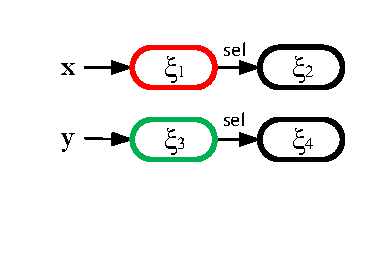
\includegraphics[page=1,scale=0.65]{../figures/fig12.pdf} & \includegraphics[page=2,scale=0.65]{../figures/fig12.pdf}\\
\end{tabular}


\end{frame}




%%%%%%%%%%%%%%%%%
% # QUESTA SI METTE O NO???
%\begin{frame}{Recap}
%We can define \textbf{ALoc} even in a different way:
%\begin{footnotesize}
%\begin{table}
%\begin{tabular}{|c|c|}
%\hline
%\textbf{Definition} & \textbf{Locations} \\
%\hline
%$\mathsf{S} \;=\; \mathcal{P}(\mathbf{Var}_* \times \mathbf{ALoc})$ & $ALoc(\mathsf{S}) = \{ n_X | \exists x : (x, n_X) \in \mathsf{S} \}$ \\
%\hline
%$\mathsf{H} \;=\; \mathcal{P}(\mathbf{ALoc} \times \mathbf{Sel} \times \mathbf{ALoc})$ & $ALoc(\mathsf{H}) = \{ n_V, n_W | \exists sel : (n_V, sel, n_W) \in \mathsf{H} \}$ \\
%\hline
%
%\end{tabular}
%\end{table}
%\end{footnotesize}
%\end{frame}

\subsection{Complete Lattice}

\begin{frame}{Summarize}

To summarize a shape graph is composed by:
\begin{alignat*}{3}
& \mathsf{S} \;\in && \; \mathbf{AState} \quad && =\quad \mathcal{P}(\mathbf{Var}_* \times \mathbf{ALoc}) \\
& \mathsf{H} \;\in && \; \mathbf{AHeap} \quad && =\quad \mathcal{P}(\mathbf{ALoc} \times \mathbf{Sel} \times \mathbf{ALoc}) \\
& \mathsf{is} \;\in && \; \mathbf{IsShared} \quad && =\quad \mathcal{P}(\mathbf{ALoc}) \\
\end{alignat*}

where

$$ \mathbf{ALoc} \; = \; \{ n_Z \;|\; Z \subseteq \mathbf{Var}_* \} $$

\end{frame}

\begin{frame}{Compatible Shape Graph}

We say that a shape graph is \textbf{compatible} if it fulfil the 5 invariants: \\
\begin{footnotesize}
\begin{enumerate}

\item $ \;\;\forall n_V, n_W \in ALoc(\textsf{S}) \cup ALoc(\textsf{H}) \cup \textsf{is} : (V = W) \vee (V \cap W = \emptyset) $

\item $ \;\;\forall (x, n_X) \in \textsf{S} : x \in X $

\item $ \;\;\forall (n_V,sel,n_W),(n_V,sel,n_{W'}) \in \textsf{H} : (V = \emptyset) \vee (W = W') $

\item $\begin{array}{ll}
\forall n_X \in \textsf{is}: & \;(\exists sel : (n_\emptyset, sel, n_X) \in \textsf{H}) \;\vee \\
\quad & \;(\exists (n_V, sel_1, n_X), (n_W, sel_2, n_X) \in \textsf{H} : \\
\quad & \;\quad\quad sel_1 \neq sel_2 \vee V \neq W )
\end{array}$

\item $\begin{array}{l}
\forall (n_V, sel_1, n_X), (n_W, sel_2, n_X) \in \textsf{H}: \\
\quad\quad ((sel_1 \neq sel_2 \vee V \neq W) \wedge X \neq \emptyset) \Rightarrow n_X \in \textsf{is} \\
\end{array}$

\end{enumerate}
\end{footnotesize}
\end{frame}

\begin{frame}{Compatible Shape Graph}

The sets of compatible shape graphs is denoted by 
$$ \mathbf{SG} = \{\textsf{(S,H,is)} \;|\; \textsf{(S,H,is)} \mathrm{\;is\;compatible} \} $$

\medskip
\pause

Our analysis will work on \emph{sets} of compatible shape graphs (elements of $\mathcal{P}(\mathbf{SG})$).

\medskip
\pause

$\mathcal{P}(\mathbf{SG})$ is trivially a \textbf{complete lattice}, with $\sqcup$ being $\cup$ and $\sqsubseteq$ being $\subseteq$.

\medskip
\pause

$\mathcal{P}(\mathbf{SG})$ is obviously \textbf{finite} because $\mathbf{SG} \subseteq \mathbf{AState} \times \mathbf{AHeap} \times \mathbf{IsShared}$, and $\mathbf{AState}$, $\mathbf{AHeap}$ and $\mathbf{IsShared}$ are \textbf{finite}.
\end{frame}

\section{The Analysis}

\begin{frame}{The Analysis}

We introduce the analysis $Shape$ as an instance of a \textbf{Monotone Framework}. For every labeled program $S_*$ we produce a sets of equations of the form.

\pause

\begin{footnotesize}
\begin{align*}
Shape_{\circ}(\ell) &= \left\{
\begin{array}{ll}
\iota  &\mathrm{if} \ell = init(S_*) \\
\bigcup \{Shape_{\bullet}(\ell') \;|\; (\ell', \ell) \in flow(S_*)\} & \mathrm{otherwise} \\
\end{array}
\right. \\
Shape_{\bullet}(\ell)  &= f_\ell^{\mathsf{SA}}(Shape_{\circ}(\ell)) 
\end{align*}
\end{footnotesize}

\pause

Where $\iota \in \mathcal{P}(\mathbf{SG})$ is the extremal value at entry of $S_*$ and $f_\ell^{SA}$ is the transfer function.

\end{frame}

\begin{frame}{The Analysis}
The analysis \emph{Shape} is a \textbf{forward analysis}, because it's defined using the set $flow(S_*)$.

\medskip
\pause

It's also a \textbf{may analysis} since we are using the $\bigcup$ operator for combining results gathered from the $flow(S_*)$.

\medskip
\pause

The \textbf{transfer function} $f_\ell^{\mathsf{SA}} : \mathcal{P}(\mathbf{SG}) \rightarrow \mathcal{P}(\mathbf{SG})$ has the form:

$$ f_\ell^{\mathsf{SA}}(SG) = \bigcup \{ {\phi}_\ell^{\mathsf{SA}} \mathsf{((S,H,is))} \;|\; \mathsf{(S,H,is)} \in SG \} $$

The function ${\phi}_\ell^{\mathsf{SA}}$ has to be developed right now.
\end{frame}

\begin{frame}{The function ${\phi}_\ell^{\mathsf{SA}}$}

The function ${\phi}_\ell^{\mathsf{SA}} : \mathbf{SG} \rightarrow \mathcal{P}(\mathbf{SG})$ specifies how a \textbf{single} graph in $Shape_{\circ}(\ell)$ is transformed into a \textbf{set} of graph in $Shape_{\bullet}(\ell)$

\medskip
\pause

We present the ${\phi}_\ell^{\mathsf{SA}}$ function for all the different kind of statements.

\end{frame}

\subsection{$[b]^\ell$ and $[\mathtt{skip}]^\ell$}

\begin{frame}{}
\begin{center}
\begin{huge}
\textcolor{bl}{$[b]^\ell$ and $[\mathtt{skip}]^\ell$}
\end{huge}
\end{center}
\end{frame}

\begin{frame}{$[b]^\ell$ and $[\mathtt{skip}]^\ell$}

Since $[b]^\ell$ and $[\mathtt{skip}]^\ell$ does \textbf{not modify} the heap, the ${\phi}_\ell^{\mathsf{SA}}$ function is just the \textbf{identity} functions, remember that we are interested in the heap shape.

\medskip
\pause

$${\phi}_\ell^{\mathsf{SA}}\mathsf{((S,H,is))} = \mathsf{ \{ (S,H,is) \} }$$

\end{frame}


\subsection{$[x:=a]^\ell$}

\begin{frame}{}
\begin{center}
\begin{huge}
\textcolor{bl}{$[x:=a]^\ell$}
\end{huge}
\end{center}
\end{frame}


\begin{frame}{$[x:=a]^\ell$}

\begin{block}{}
We consider $[x:=a]^\ell$ in the case where $a$ is of the form $n$, $a_1 \; op_a \; a_2$ or \texttt{nil}.
\end{block}

\medskip
\pause

We must \textbf{remove the binding} of $x$ and \textbf{rename} all the abstract location that contains $x$.

$$ k_x (n_Z) = n_{Z \backslash \{ x \}} $$

\medskip
\pause

So we take 
$${\phi}_\ell^{\mathsf{SA}}\mathsf{((S,H,is))} = \{ kill_x \mathsf{ (S,H,is) } \} $$

\end{frame}

\begin{frame}{$[x:=a]^\ell$}

Where $kill_x \mathsf{ (S,H,is) } = \mathsf{(S', H', is')}$ is given by

\begin{align*}
\mathsf{S'} \; &= \; \{ (z, k_x(n_Z) )\;|\; (z, n_Z) \in \mathsf{S} \wedge z \neq x \} \\
\medskip
\mathsf{H'} \; &= \; \{ (k_x(n_V), sel, k_x(n_W)) \;|\; (n_V, sel, n_W) \in \mathsf{H} \} \\
\medskip
\mathsf{is'} \; &= \; \{ (k_x(n_X) )\;|\; n_X \in \mathsf{is} \}
\end{align*}

\medskip
\pause

It's easy to prove that if $\mathsf{(S,H,is)}$ is compatible, even $\mathsf{(S',H',is')}$ is compatible.

\end{frame}

\begin{frame}{If $(x, n_{ \{ x \} })$ is in \textbf{S}?}

If $(x, n_{ \{ x \} })$ is in \textbf{S} then the two abstract location $n_{\{x\}}$ and $n_\emptyset$ will be \textbf{merged}.

\medskip
\pause

From this we can deduce that $n_\emptyset$ will be \textbf{unshared} if \textbf{both} $n_{ \{ x \} }$ and $n_\emptyset$ was \textbf{unshared}.

\medskip
\pause

\begin{block}{Garbage Collection}
Please note that our analysis does not provide a \textbf{garbage collector}, so if $n_{ \{ x \} }$ has no heap pointer, it is \textbf{unreachable}.

Consider that there will be a pointer from $n_\emptyset$ to the location that $n_{ \{ x \} }$ might point to.  

\end{block}
\end{frame}

\begin{frame}[fragile]{$[x:=a]^\ell$}
\begin{center}

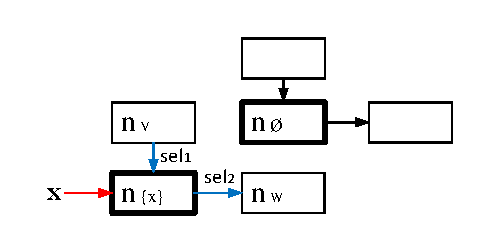
\includegraphics[page=1,scale=0.8]{../figures/fig5.pdf}\\
$\mathsf{(S,H,is)}$\\
\medskip
\includegraphics[page=2,scale=0.8]{../figures/fig5.pdf}\\
$\mathsf{(S',H',is')}$\\

\end{center}
\end{frame}

\subsection{$[x:=y]^\ell$}

\begin{frame}{}
\begin{center}
\begin{huge}
\textcolor{bl}{$[x:=y]^\ell$}
\end{huge}
\end{center}
\end{frame}




\begin{frame}{$[x:=y]^\ell$}

if $x = y$ the $f_\ell^{\textsf{SA}}$ is just the identity function.

\medskip
\pause

if $x \neq y$ then we execute the following steps:
\begin{enumerate}
\item We remove the old binding for $x$ with $kill_x$,
\item We update the abstract location that contains $y$ adding $\{ x \}$ to the variable sets.
\end{enumerate}

\medskip
\pause

This can be done with
$$g_x^y (n_Z) = \left \{
\begin{array}{ll}
n_{Z \cup \{ x \} } & \mathrm{if}\; y \in Z \\
n_Z & \mathrm{otherwise}
\end{array}
\right.
$$

\end{frame}

\begin{frame}{$[x:=y]^\ell$}

So we take 
$${\phi}_\ell^{\mathsf{SA}}\mathsf{((S,H,is))} = \{ \mathsf{ (S'',H'',is'') } \} $$
Where $\mathsf{(S', H', is')} = kill_x (\mathsf{(S,H,is)})$ and

\pause

\begin{align*}
\mathsf{S''} \; &= \; \{ (z, g_x^y(n_Z)) \;|\; (z, n_Z) \in \mathsf{S'} \} \\
&\;\;\quad \cup \{ (x, g_x^y(n_Y)) \;|\; (y', n_Y) \in \mathsf{S'} \wedge y' = y\} \\
\mathsf{H''} \; &= \; \{ (g_x^y(n_V), sel, g_x^y(n_W)) \;|\; (n_V, sel, n_W) \in \mathsf{H'} \} \\
\medskip
\mathsf{is''} \; &= \; \{ g_x^y(n_Z) \;|\; n_Z \in \mathsf{is'} \}
\end{align*}

\medskip
\pause

Again it's easy to prove that if $\mathsf{(S,H,is)}$ is compatible, even $\mathsf{(S'',H'',is'')}$ is compatible.

\end{frame}

\begin{frame}{$[x:=y]^\ell$}

\begin{align*}
\mathsf{S''} \; &= \; \{ (z, g_x^y(n_Z)) \;|\; (z, n_Z) \in \mathsf{S'} \} \\
&\;\;\quad \cup \textcolor{bl}{\{ (x, g_x^y(n_Y)) \;|\; (y', n_Y) \in \mathsf{S'} \wedge y' = y\}} \\
\mathsf{H''} \; &= \; \{ (g_x^y(n_V), sel, g_x^y(n_W)) \;|\; (n_V, sel, n_W) \in \mathsf{H'} \} \\
\medskip
\mathsf{is''} \; &= \; \{ g_x^y(n_Z) \;|\; n_Z \in \mathsf{is'} \}
\end{align*}

\begin{block}{}

Please note that the clause in blue is the \textbf{adding} of the binding of $x$.
\\
The sharing information of $n_{Y \cup \{ x \} }$ in inherited from $n_Y$.

\end{block}

\end{frame}

\begin{frame}[fragile]{$[x:=y]^\ell$}
A little example when $x \neq y$.
\begin{center}
\includegraphics<1>[page=1]{../figures/fig6.pdf}
\only<1>{\\$\mathsf{(S,H,is)}$}
\includegraphics<2>[page=2]{../figures/fig6.pdf}
\only<2>{\\$\mathsf{(S'',H'',is'')}$}
\end{center}
\end{frame}

\subsection{$[x:=y.sel]^\ell$}

\begin{frame}{}
\begin{center}
\begin{huge}
\textcolor{bl}{$[x:=y.sel]^\ell$}
\end{huge}
\end{center}
\end{frame}



\begin{frame}{$[x:=y.sel]^\ell$}

If $x = y$ the assignment is equivalent to:
$$[t:=y.sel]^{\ell_1};\; [x:=t]^{\ell_2};\; [t:=\mathtt{nil}]^{\ell_3};\; $$

Where $t$ is a \textbf{fresh variable} and $\ell_1$, $\ell_2$ and $\ell_3$ are \textbf{fresh labels}.\\

\medskip
\pause

We can obtain the transfer function $f_\ell^{\textsf{SA}}$ as a \textbf{composition}:
$$f_\ell^{\textsf{SA}} = f_{\ell_3}^{\textsf{SA}} \circ f_{\ell_2}^{\textsf{SA}} \circ f_{\ell_1}^{\textsf{SA}}$$

So $f_{\ell_2}^{\textsf{SA}}$ and $f_{\ell_3}^{\textsf{SA}}$ can be computed using the same pattern as before. We concentrate on $f_{\ell_1}^{\textsf{SA}}$ (or similar in the case when $x \neq y$).

\end{frame}

\begin{frame}{$[x:=y.sel]^\ell$}

First of all we remove the old binding for $x$:
$$ \mathsf{(S', H', is')} = kill_x (\mathsf{(S,H,is)})$$

\pause

Then we must rename the abstract location corresponding to $y.sel$ to include $x$ into the variable set, then we must add the new binding for $x$. We can have 3 different cases:

\pause

\begin{enumerate}
\item There is no abstract location $n_Y$ such that $(y, n_Y) \in \mathsf{S'}$, or  it exist but there is no $n_Z$ such that $(n_Y, sel, n_Z) \in \mathsf{H'}$. 
\pause
\item There is an abstract location $n_Y$ such that $(y, n_Y) \in \mathsf{S'}$ and there is a $n_U \neq n_\emptyset$ such that $(n_Y, sel, n_U) \in \mathsf{H'}$. 
\pause
\item There is an abstract location $n_Y$ such that $(y, n_Y) \in \mathsf{S'}$ and there is a triple such that $(n_Y, sel, n_\emptyset) \in \mathsf{H'}$. 
\end{enumerate}
\end{frame}

\subsubsection{Case 1}
\begin{frame}{$[x:=y.sel]^\ell$ - Case 1}
In the case where there is no abstract location $n_Y$ such that $(y, n_Y) \in \mathsf{S'}$ we simply take:

$$ \phi_{\ell}^{\mathsf{SA}}(\mathsf{(S, H, is)}) = kill_x (\mathsf{(S,H,is)})$$

\pause
\medskip

In the case where there is no $n_Z$ such that $(n_Y, sel, n_Z) \in \mathsf{H'}$ we again take 

$$ \phi_{\ell}^{\mathsf{SA}}(\mathsf{(S, H, is)}) = kill_x (\mathsf{(S,H,is)})$$

\pause
\medskip

\begin{block}{}
In both case there is no binding to add, so we simply remove the old binding for $x$. The first case is the case of de-referencing of \texttt{nil}-pointer, the second case is the case of de-referencing of non-existing fields.
\end{block}
\end{frame}

\subsubsection{Case 2}
\begin{frame}{$[x:=y.sel]^\ell$ - Case 2}

We consider the case where there is an abstract location $n_Y$ such that $(y, n_Y) \in \mathsf{S'}$ and there is a $n_U \neq n_\emptyset$ such that $(n_Y, sel, n_U) \in \mathsf{H'}$. 

\medskip
\pause

We must rename $n_U$ to include $x$ into the variable set using the function:

$$h_x^U (n_Z) = \left \{
\begin{array}{ll}
n_{Z \cup \{ x \} } & \mathrm{if}\; Z = U \\
n_Z & \mathrm{otherwise}
\end{array}
\right.
$$

\end{frame}

\begin{frame}{$[x:=y.sel]^\ell$ - Case 2}

So we take 
$${\phi}_\ell^{\mathsf{SA}}\mathsf{((S,H,is))} = \{ \mathsf{ (S'',H'',is'') } \} $$
Where $\mathsf{(S', H', is')} = kill_x (\mathsf{(S,H,is)})$ and

\pause

\begin{align*}
\mathsf{S''} \; &= \; \{ (z, h_x^U(n_Z)) \;|\; (z, n_Z) \in \mathsf{S'} \} \cup \{ (x, h_x^U(n_U)) \} \\
\mathsf{H''} \; &= \; \{ (h_x^U(n_V), sel, h_x^U(n_W)) \;|\; (n_V, sel, n_W) \in \mathsf{H'} \} \\
\medskip
\mathsf{is''} \; &= \; \{ h_x^U(n_Z) \;|\; n_Z \in \mathsf{is'} \}
\end{align*}
\end{frame}

\begin{frame}{$[x:=y.sel]^\ell$ - Case 2}

$$ \mathsf{S''} \; = \; \{ (z, h_x^U(n_Z)) \;|\; (z, n_Z) \in \mathsf{S'} \} \cup \textcolor{bl}{ \{ (x, h_x^U(n_U)) \} } $$

\begin{block}{}
The clause in blue represent the adding of the new binding for $x$.
\\
\medskip

As before $n_{U \cup \{ x \}}$ is shared in $\mathsf{(H'')}$ if and only if $n_U$ was shared in $\mathsf{(H')}$.

\end{block}

\end{frame}

\begin{frame}{$[x:=y.sel]^\ell$ - Case 2}
Let's show this case with a little example when $x \neq y$, and in case when $n_U \in \mathsf{is}$.

\begin{center}
\includegraphics<1>[page=1]{../figures/fig7.pdf}
\only<1>{\\$\mathsf{(S,H,is)}$}
\includegraphics<2>[page=2]{../figures/fig7.pdf}
\only<2>{\\$\mathsf{(S'',H'',is'')}$}
\end{center}
\end{frame}

\subsubsection{Case 3}
\begin{frame}{$[x:=y.sel]^\ell$ - Case 3}

Consider now the case where there is an abstract location $n_Y$ such that $(y, n_Y) \in \mathsf{S'}$ and there is a triple such that $(n_Y, sel, n_\emptyset) \in \mathsf{H'}$. 

\medskip
\pause

The location for $y.sel$ is represented by $n_\emptyset$ (that represent even other locations). We must \textbf{materialize} an abstract location $n_{ \{ x \} }$ from $n_\emptyset$, doing so $n_{ \{ x \}}$ will represent $y.sel$ and $n_\emptyset$ will represent the remaining locations.

\medskip
\pause

This operation is a bit hard so let's consider an example

\end{frame}

\begin{frame}[fragile]{$[x:=y.sel]^\ell$ - Case 3}

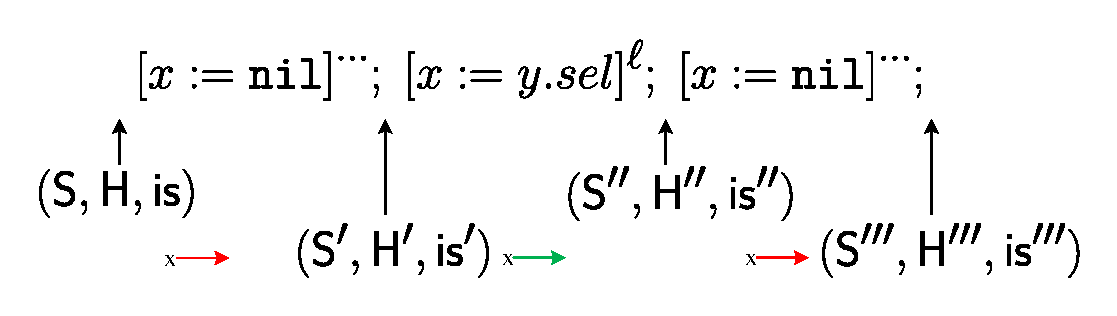
\includegraphics[scale=0.5]{../figures/fig11.pdf}

\pause
We can determinate obviously that
\begin{itemize}
\item $[x:=\mathtt{nil}]^{\cdots};\;[x:=y.sel]^{\ell}$ is equivalent to $[x:=y.sel]^{\ell}$
\pause
\item $\mathsf{(S',H',is')} = kill_x \mathsf{((S,H,is))}$ 
\pause
\item $\mathsf{(S''',H''',is''')} = kill_x \mathsf{((S'',H'',is''))}$ 
\pause
\item $\mathsf{(S''',H''',is''')} = \mathsf{(S',H',is')} $
\end{itemize}
\end{frame}

\begin{frame}{$[x:=y.sel]^\ell$ - Case 3}

So finally $$kill_x \mathsf{((S'',H'',is''))} = \mathsf{(S',H',is')}$$
Then we can also say that $(x, n_{ \{x\} }) \in \mathsf{S''}$ and that $(n_Y, sel, n_{ \{ x \} }) \in \mathsf{H''}$.

\medskip
\pause

So we can take
\begin{block}{}
\begin{align*}
\phi_{\ell}^{\mathsf{SA}}((\mathsf{S,H,is})) \;=\;  \{&(\mathsf{S'',H'',is''}) \;|\;\\
&(\mathsf{S'',H'',is''}) \mathrm{\;is\;compatible\;} \;\wedge \\
&kill_x ((\mathsf{S'',H'',is''})) = (\mathsf{S',H',is'}) \;\wedge \\
&(x, n_{ \{x\} }) \in \mathsf{S''} \;\wedge\; (n_Y, sel, n_{ \{ x \} }) \in \mathsf{H''} \}
\end{align*}
\end{block}
\end{frame}

\begin{frame}{$[x:=y.sel]^\ell$ - Case 3}

We are sure that we have included all the possible solutions. So our function is \textbf{sound}.

\medskip
\pause

Is it possible that we have included too much solutions, so we are \textbf{losing precision}?

\medskip
\pause

We will now argue that the amount of imprecision in \textbf{not excessive}.

\end{frame}

\begin{frame}[fragile]{$[x:=y.sel]^\ell$ - Case 3}

First we prove that $$ \mathsf{S'' = S'} \cup \{(x, n_{ \{x\} }) \} $$ \\

\pause

\begin{block}{Proof}

\begin{footnotesize}

\begin{description}
\item[$ \mathsf{S'' \subseteq S'} \cup \{(x, n_{ \{x\} }) \}  $] Consider $(z, n_Z) \in \mathsf{S''}$. If $z = x$ then from compatibility $n_Z = n_{ \{x\} }$. If $z \neq x$ then from $(x, n_{ \{x\} }) \in \mathsf{S''}$ and the compatibility we deduce that $x \not\in Z$ and so $(z, n_Z) = (z, k_x (n_Z))$ (and $k_x$ is used to define $kill_x$).\\
\item[$  \mathsf{S'' \supseteq S'} \cup \{(x, n_{ \{x\} }) \}  $] Consider $(u, n_U) \in \mathsf{S'}$. We know from definition of $\mathsf{S'}$ and from compatibility that $u \neq x$ and $x \not\in U$. There must be a $(u, n'_{U}) \in \mathsf{S''}$ such that $k_x(n'_U) = n_U$, but since $x \neq y$ we obtain $n'_U = n_U$.\\
\end{description}

\begin{flushright}
$\square$
\end{flushright}
\end{footnotesize}

\end{block}

\end{frame}


\begin{frame}{$[x:=y.sel]^\ell$ - Case 3}

Then we prove that
\begin{align*}
\mathsf{is'} \backslash \{ n_\emptyset \} \quad=&\quad \mathsf{is''} \backslash \{ n_\emptyset, n_{\{ x \}} \} \\
n_\emptyset \in \mathsf{is'} \quad\mathrm{iff}&\quad n_\emptyset \in \mathsf{is''} \vee n_{\{ x \}} \in \mathsf{is''}
\end{align*} 

\medskip
\pause

Equal as showing that
\begin{itemize}
\item Sharing information of location apart $n_\emptyset$ are conserved,
\item If $n_\emptyset$ is shared then it can rise share to $n_\emptyset$ or to $n_{\{ x \}}$ (or both),
\item If $n_\emptyset$ is not shared, we can't introduce a sharing for $n_\emptyset$ neither for $n_{\{ x \}}$.
\end{itemize}

\end{frame}

\begin{frame}{$[x:=y.sel]^\ell$ - Case 3}

Then we prove that
\begin{align*}
\mathsf{is'} \backslash \{ n_\emptyset \} \quad=&\quad \mathsf{is''} \backslash \{ n_\emptyset, n_{\{ x \}} \} \\
n_\emptyset \in \mathsf{is'} \quad\mathrm{iff}&\quad n_\emptyset \in \mathsf{is''} \vee n_{\{ x \}} \in \mathsf{is''}
\end{align*} 

\medskip
\pause

\begin{block}{Proof}
\begin{footnotesize}
Since $\mathsf{(S',H',is')}$ and $\mathsf{(S'',H'',is'')}$ are compatible, if $n_U \in \mathsf{is'}$ then $x \not\in U$ and if $n_U \in \mathsf{is''}$ then $x \not\in U \vee \{ x \} = U$.\\

\medskip

Remember that $\mathsf{is'} = \{ k_x(n_U) \;|\; n_U \in \mathsf{is''} \} $, so we can deduce that $\mathsf{is'} \backslash \{ n_\emptyset \} = \mathsf{is''} \backslash \{n_\emptyset, n_{\{x\}} \}$, because $k_x(n_U) = n_U \neq n_\emptyset$ for all $n_U \in \mathsf{is''} \backslash \{n_\emptyset, n_{\{x\}} \}$.\\

\medskip

More $n_\emptyset \in \mathsf{is''} \vee n_{\{x\}} \in \mathsf{is''} \Rightarrow n_\emptyset \in \mathsf{is'}$ and more $n_\emptyset \not\in \mathsf{is''} \wedge n_{\{x\}} \not\in \mathsf{is''} \Rightarrow n_\emptyset \not\in \mathsf{is'}$

\begin{flushright}
$\square$
\end{flushright}
\end{footnotesize}
\end{block}

\end{frame}


\begin{frame}{$[x:=y.sel]^\ell$ - Case 3}

Now consider the abstract heap H, we first classify the edge depending on if the source and the target are either $n_\emptyset$ or $n_{\{x\}}$.

\pause

\begin{footnotesize}

\begin{align*}
(n_V, sel', n_W)\; \mathrm{is}\; external \quad\mathrm{iff}&\quad \{n_V, n_W\} \cap \{n_\emptyset, n_{\{x\}}\} = \emptyset \\
(n_V, sel', n_W)\; \mathrm{is}\; internal \quad\mathrm{iff}&\quad \{n_V, n_W\} \subseteq \{n_\emptyset, n_{\{x\}}\} \\
(n_V, sel', n_W)\; \mathrm{is}\; going\text{-}out \quad\mathrm{iff}&\quad n_V \in \{n_\emptyset, n_{\{x\}} \} \wedge n_W \not\in \{n_\emptyset, n_{\{x\}} \} \\
(n_V, sel', n_W)\; \mathrm{is}\; going\text{-}in \quad\mathrm{iff}&\quad n_V \not\in \{n_\emptyset, n_{\{x\}}\} \wedge n_W \in \{n_\emptyset, n_{\{x\}} \} \\
\end{align*}

\pause

We say that two edge $(n_V, sel', n_W)$ and $(n'_V, sel'', n'_W)$ are \textbf{related} if and only if $k_x(n_V) = k_x(n'_V)$, $sel' = sel''$ and $k_x(n_W) = k_x(n'_W)$.

\end{footnotesize}
\end{frame}

\begin{frame}{$[x:=y.sel]^\ell$ - Case 3}

We can show that
\begin{itemize}
\item $\mathsf{H'}$ and $\mathsf{H''}$ have the same external edges,
\pause
\medskip
\item each internal edge in $\mathsf{H'}$ is related to an internal edge in $\mathsf{H''}$ and vice versa,
\pause
\medskip
\item each going-out edge in $\mathsf{H'}$ is related to a going-out edge in $\mathsf{H''}$ and vice versa,
\pause
\medskip
\item each going-in edge in $\mathsf{H'}$ is related to a going-in edge in $\mathsf{H''}$ and vice versa,
\end{itemize}
\pause
Obviously the edge $(n_Y, sel, n_\emptyset) \in \mathsf{H'}$ must be update with $(n_Y, sel, n_{\{x\}}) \in \mathsf{H''}$. We impose that $(n_Y, sel, n_{\{x\}}) \in \mathsf{H''}$, and because of compatibility we deduce that $(n_Y, sel, n_{\{x\}}) \not\in \mathsf{H'}$.
\end{frame}

\begin{frame}{$[x:=y.sel]^\ell$ - Case 3}

Consider the following scenario and let's see what happens after $[x:=y.sel]^\ell$.

\includegraphics[page=3]{../figures/fig7.pdf}
$$\mathsf{(S,H,is)}$$

\end{frame}

\begin{frame}{$[x:=y.sel]^\ell$ - Case 3}

We extract the location $n_X$ from $n_\emptyset$, and depending on the triple involving $sel_2$ and $sel_3$ we can have 6 different and compatible shape graphs.

\includegraphics[page=7]{../figures/fig8.pdf}

$$\mathsf{(S'',H'',is'')}$$
\end{frame}


\begin{frame}{$[x:=y.sel]^\ell$ - Case 3}

\includegraphics<1>[page=1]{../figures/fig8.pdf}
\includegraphics<2>[page=2]{../figures/fig8.pdf}
\includegraphics<3>[page=3]{../figures/fig8.pdf}
\includegraphics<4>[page=4]{../figures/fig8.pdf}
\includegraphics<5>[page=5]{../figures/fig8.pdf}
\includegraphics<6>[page=6]{../figures/fig8.pdf}
\only<1>{$$\mathsf{(S''_1,H''_1,is''_1)}$$}
\only<2>{$$\mathsf{(S''_2,H''_2,is''_2)}$$}
\only<3>{$$\mathsf{(S''_3,H''_3,is''_3)}$$}
\only<4>{$$\mathsf{(S''_4,H''_4,is''_4)}$$}
\only<5>{$$\mathsf{(S''_5,H''_5,is''_5)}$$}
\only<6>{$$\mathsf{(S''_6,H''_6,is''_6)}$$}

\end{frame}

\subsection{$[x.sel:=a]^\ell$}

\begin{frame}{}
\begin{center}
\begin{huge}
\textcolor{bl}{$[x.sel:=a]^\ell$}
\end{huge}
\end{center}
\end{frame}


\begin{frame}{$[x.sel:=a]^\ell$}

\begin{block}{}
We consider $[x.sel:=a]^\ell$ in the case where $a$ is of the form $n$, $a_1 \; op_a \; a_2$ or \texttt{nil}.
\end{block}
Let's consider a compatible graph $\mathsf{(S,H,is)}$. \\
\medskip
\pause
The easy case are:
\begin{itemize}
\begin{small}
\item The case where there is no $n_X$ such that $(x, n_X) \in \mathsf{S}$, the statement will have no effect ($x$ does not point to a cell in the heap). In this case the transfer function $f_\ell^{\mathsf{SA}}$ is just the identity.
\medskip
\pause
\item The case where there is a $n_X$ such that $(x, n_X) \in \mathsf{S}$, but there is no $n_U$ such that $(n_X, sel, n_U) \in \mathsf{H}$; even in this case the statement will have no effect (the cell pointed by $sel$ does not point to another cell in the heap). In this case the transfer function $f_\ell^{\mathsf{SA}}$ is again the identity.
\end{small}
\end{itemize}
\end{frame}

\begin{frame}{$[x.sel:=a]^\ell$}
Consider the case where there is a $n_X$ such that $(x, n_X) \in \mathsf{S}$ and there is a unique $n_U$ such that $(n_X, sel, n_U) \in \mathsf{H}$.

\medskip
\pause

The effect will be to \textbf{remove} the triple $(n_X, sel, n_U)$:
$${\phi}_\ell^{\mathsf{SA}}\mathsf{((S,H,is))} = \{ kill_{x.sel} \mathsf{ (S,H,is) } \} $$


\end{frame}

\begin{frame}{$[x.sel:=a]^\ell$}
$${\phi}_\ell^{\mathsf{SA}}\mathsf{((S,H,is))} = \{ kill_{x.sel} \mathsf{ (S,H,is) } \} $$
\\
\medskip
where $kill_{x.sel} \mathsf{ (S,H,is) = (S', H', is')} $ is given by
\pause
\begin{align*}
\mathsf{S'} \quad=&\quad \mathsf{S} \\
\mathsf{H'} \quad=&\quad \{ (n_V, sel',n_W) | (n_V, sel', n_W) \in \mathsf{H} \;\wedge\\
&\;\quad \neg(X = V \wedge sel = sel') \} \\
\mathsf{is'} \quad=&\quad \left\{
\begin{array}{ll}
\mathsf{is} \backslash \{n_U\} & \mathrm{if}\; n_U \in \mathsf{is} \;\wedge\; \#into(n_U,\mathsf{H'}) \leq 1 \;\wedge\; \\
&\quad \neg \exists sel' : (n_\emptyset, sel', n_U) \in \mathsf{H'}\\
\mathsf{is} & \mathrm{otherwise} \\
\end{array}
\right.
\end{align*} 

\end{frame}

\begin{frame}{$[x.sel:=a]^\ell$}
$$
\mathsf{is'} \quad=\quad \left\{
\begin{array}{ll}
\mathsf{is} \backslash \{n_U\} & \mathrm{if}\; n_U \in \mathsf{is} \;\wedge\; \textcolor{bl}{\#into(n_U,\mathsf{H'})} \leq 1 \;\wedge\; \\
&\quad \neg \exists sel' : (n_\emptyset, sel', n_U) \in \mathsf{H'}\\
\mathsf{is} & \mathrm{otherwise} \\
\end{array}
\right.
$$

\medskip
\pause 

We use $\#into(n_U,\mathsf{H'})$ to indicate the number of pointer to $n_U$ in $\mathsf{H'}$. 

\medskip

With the first clause we check if it is possible to remove $n_U$ from is. If the number of pointers to $n_U$ is less then 2 and there is no $(n_\emptyset, sel', n_U)$ triple in $\mathsf{H'}$ then we can remove it.
\end{frame}

\begin{frame}{$[x.sel:=a]^\ell$}

Let's view the effect of $[x.sel:=\mathtt{nil}]^\ell$ when $\#into(n_U, \mathsf{H'}) \leq 1$.

\begin{center}
\includegraphics<1>[page=1]{../figures/fig9.pdf}
\only<1>{\\$\mathsf{(S,H,is)}$}
\includegraphics<2>[page=2]{../figures/fig9.pdf}
\only<2>{\\$\mathsf{(S',H',is')}$}
\end{center}
\end{frame}


\subsection{$[x.sel:=y]^\ell$}

\begin{frame}{}
\begin{center}
\begin{huge}
\textcolor{bl}{$[x.sel:=y]^\ell$}
\end{huge}
\end{center}
\end{frame}



\begin{frame}{$[x.sel:=y]^\ell$}

If $x = y$ the assignment is equivalent to:
$$[t:=y]^{\ell_1};\; [x.sel:=t]^{\ell_2};\; [t:=\mathtt{nil}]^{\ell_3};\; $$

Where $t$ is a \textbf{fresh variable} and $\ell_1$, $\ell_2$ and $\ell_3$ are \textbf{fresh labels}.\\

\medskip
\pause

We can obtain the transfer function $f_\ell^{\textsf{SA}}$ as a \textbf{composition}:
$$f_\ell^{\textsf{SA}} = f_{\ell_3}^{\textsf{SA}} \circ f_{\ell_2}^{\textsf{SA}} \circ f_{\ell_1}^{\textsf{SA}}$$

So $f_{\ell_1}^{\textsf{SA}}$ and $f_{\ell_3}^{\textsf{SA}}$ can be computed using the same pattern as before. We concentrate on $f_{\ell_2}^{\textsf{SA}}$ (or similar in the case when $x \neq y$).

\end{frame}

\begin{frame}{$[x.sel:=y]^\ell$}

Assume $x \neq y$ and let $\mathsf{(S,H,is)}$ be a compatible shape graph.

\medskip
\pause

In the case where there is no $n_X$ such that $(x, n_X) \in \mathsf{S}$ then the $f_\ell^{\textsf{SA}}$ is just the identity function.

\medskip
\pause

Consider the case where there is a $n_X$ such that $(x, n_{X}) \in \mathsf{S}$, but there is no $n_Y$ such that $(y, n_{Y}) \in \mathsf{S}$. It's the case where $y$ is an integer value, or the \texttt{nil} value, it can be treated as $[x.sel:=a]^\ell$:

$${\phi}_\ell^{\mathsf{SA}}\mathsf{((S,H,is))} = \{ kill_{x.sel} \mathsf{ (S,H,is) } \} $$

\end{frame}

\begin{frame}{$[x.sel:=y]^\ell$}
In the case where $x \neq y$, $(x, n_X) \in \mathsf{S}$ and $(y, n_Y) \in \mathsf{S}$ we proceed with 2 steps.
\pause
\medskip
\begin{enumerate}
\item First we remove the binding for $x.sel$,
\item Then we add the new binding.
\end{enumerate}
\end{frame}

\begin{frame}{$[x.sel:=y]^\ell$}
$${\phi}_\ell^{\mathsf{SA}}\mathsf{((S,H,is))} = \{ \mathsf{ (S'',H'',is'') } \} $$
\medskip
where $\mathsf{ (S',H',is') } = kill_{x.sel}(\mathsf{ (S,H,is) })$ and
\pause
\begin{align*}
\mathsf{S''} \quad=&\quad \mathsf{S'} \quad (=\mathsf{S}) \\
\mathsf{H''} \quad=&\quad \mathsf{H'} \cup \{(n_X, sel, n_Y)\} \\
\mathsf{is''} \quad=&\quad \left\{
\begin{array}{ll}
\mathsf{is'} \cup \{n_Y\} & \mathrm{if}\; \#into(n_Y,\mathsf{H'}) \geq 1 \\
\mathsf{is'} & \mathrm{otherwise} \\
\end{array}
\right.
\end{align*} 

Note that node $n_Y$ can become shared if we add a new edge pointing to it.

\end{frame}

\begin{frame}{$[x.sel:=y]^\ell$}

Let's view the effect of $[x.sel:=y]^\ell$ when $\#into(n_Y, \mathsf{H'}) < 1$.

\begin{center}
\includegraphics<1>[page=1]{../figures/fig10.pdf}
\only<1>{\\$\mathsf{(S,H,is)}$}
\includegraphics<2>[page=2]{../figures/fig10.pdf}
\only<2>{\\$\mathsf{(S'',H'',is'')}$}
\end{center}
\end{frame}


\subsection{$[x.sel:=y.sel']^\ell$}

\begin{frame}{}
\begin{center}
\begin{huge}
\textcolor{bl}{$[x.sel:=y.sel']^\ell$}
\end{huge}
\end{center}
\end{frame}

\begin{frame}{$[x.sel:=y.sel']^\ell$}

The statement is equivalent to:
$$[t:=y.sel']^{\ell_1};\; [x.sel:=t]^{\ell_2};\; [t:=\mathtt{nil}]^{\ell_3};\; $$

Where $t$ is a \textbf{fresh variable} and $\ell_1$, $\ell_2$ and $\ell_3$ are \textbf{fresh labels}.\\

\medskip
\pause

We can obtain the transfer function $f_\ell^{\textsf{SA}}$ as a \textbf{composition}:
$$f_\ell^{\textsf{SA}} = f_{\ell_3}^{\textsf{SA}} \circ f_{\ell_2}^{\textsf{SA}} \circ f_{\ell_1}^{\textsf{SA}}$$

So $f_{\ell_1}^{\textsf{SA}}$, $f_{\ell_2}^{\textsf{SA}}$ and $f_{\ell_3}^{\textsf{SA}}$ follow the pattern that we have seen before in the other cases.

\end{frame}

\subsection{$[\mathtt{malloc}\;x]^\ell$}

\begin{frame}{}
\begin{center}
\begin{huge}
\textcolor{bl}{$[\mathtt{malloc}\;x]^\ell$}
\end{huge}
\end{center}
\end{frame}


\begin{frame}{$[\mathtt{malloc}\;x]^\ell$}

We remove the binding for $x$ (using $kill_x$) and then we introduce a new (unshared) location pointed by $x$.

\medskip
\pause

$${\phi}_\ell^{\mathsf{SA}}\mathsf{((S,H,is))} = \{ (\mathsf{S'} \cup \{(x, n_{\{x\}})\}, \mathsf{H'}, \mathsf{is'})\} $$
\medskip
where $\mathsf{ (S',H',is') } = kill_{x}(\mathsf{ (S,H,is) })$.


\end{frame}

\subsection{$[\mathtt{malloc}\;x.sel]^\ell$}

\begin{frame}{}
\begin{center}
\begin{huge}
\textcolor{bl}{$[\mathtt{malloc}\;x.sel]^\ell$}
\end{huge}
\end{center}
\end{frame}



\begin{frame}{$[\mathtt{malloc}\;x.sel]^\ell$}
The statement is equivalent to:
$$[\mathtt{malloc}\;t]^{\ell_1};\; [x.sel:=t]^{\ell_2};\; [t:=\mathtt{nil}]^{\ell_3};\; $$

Where $t$ is a \textbf{fresh variable} and $\ell_1$, $\ell_2$ and $\ell_3$ are \textbf{fresh labels}.\\

\medskip
\pause

We can obtain the transfer function $f_\ell^{\textsf{SA}}$ as a \textbf{composition}:
$$f_\ell^{\textsf{SA}} = f_{\ell_3}^{\textsf{SA}} \circ f_{\ell_2}^{\textsf{SA}} \circ f_{\ell_1}^{\textsf{SA}}$$

So $f_{\ell_1}^{\textsf{SA}}$, $f_{\ell_2}^{\textsf{SA}}$ and $f_{\ell_3}^{\textsf{SA}}$ follow the pattern that we have seen before in the other cases.
\end{frame}


\end{document}
